\documentclass[../ManualeSviluppatore.tex]{subfiles}

\begin{document}
\section{Architettura applicazione}

	\subsection{Pattern architetturale MVP}
	\begin{figure}[!h]
		\centering
		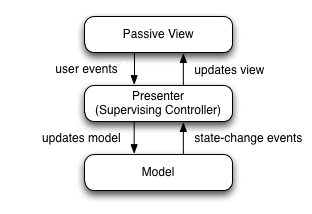
\includegraphics[scale=0.6]{img/mvp}
			\caption{Struttura del pattern MVP}
		\label{fig:StrutturaMVP}
	\end{figure}
	
			Model-View-Presenter (MVP) è un pattern architetturale derivato dal MVC (Model-View-Controller), utilizzato per dividere il codice in funzionalità distinte. 
			
			Il suo principale ambito di utilizzo è nelle applicazioni in cui sia necessario separare la logica dei componenti visivi della GUI dai componenti stessi consentendo così l'uso di diversi linguaggi per le due cose. Per esempio  descrivere le componenti in XML e definirne la logica in \gls{Java}.
			
			\subsubsection{Componenti}
			Il pattern è basato sul principio di disaccoppiamento di tre oggetti distinti, riducendo in questo modo le dipendenze reciproche; inoltre permette di fornire una maggiore modularità, manutenibilità e robustezza al \gls{software}.
				\paragraph*{Model}
					Il Model rappresenta il cuore dell'applicazione: esso definisce il modello dei dati definendo gli oggetti secondo la logica di utilizzo dell'applicazione, ossia la sua business logic. Inoltre, indica le possibili operazioni che si possono effettuare sui dati.
					
				\paragraph*{View}
					Nel pattern MVP, la View è un componente passivo che si occupa essenzialmente di notificare al Presenter eventuali interazioni con l'eventuale utente. È compito del Presenter raccogliere questi segnali ed elaborarli.
					
				\paragraph*{Presenter}
					Il Presenter è l'intermediario tra il Model e la View. Si occupa di implementare l'insieme di operazioni eseguibili sul modello dei dati attraverso una particolare vista, ossia l'application logic. Solitamente ad ogni componente della View corrisponde un componente del Presenter.
					
			\subsubsection{Vantaggi}
				Il pattern MVP per l'architettura dell'applicazione CLIPS è stato scelto perché:
				\begin{itemize}
					\item Consente di separare completamente l'interfaccia grafica dalla logica e quindi di utilizzare il linguaggio XML per descrivere l'interfaccia dell'applicazione;
					\item La completa separazione di View e Presenter consente maggiore flessibilità nella manutenzione e nell'eventuale modifica dell'interfaccia grafica;
					\item È considerato dalla comunità \gls{Android} il pattern di riferimento per un'applicazione \gls{Android};
					\item Mantiene tutti i vantaggi offerti dal pattern Model View Controller della separazione logica dei componenti.
				\end{itemize}
	
	
	\subsection{Gestione dipendenze ed estensibilità}
		Durante la progettazione dell'applicativo oltre a seguire il pattern Model View Presenter si è cercato di mantenere divisi i contratti delle classi e l'implementazione concreta attraverso l'uso di \textbf{interfacce} e delle sue implementazioni.
		Inoltre si è utilizzata la \textbf{Dependency Injection} che permette un completo disaccoppiamento tra le componenti del Model e del Presenter e garantisce che alcune componenti del Model siano Singleton.
		
	\subsection{Dependency Injection}
		\subsubsection{Dichiarazione delle dipendenze}
	Le dipendenze devono essere dichiarate annotando con \lstinline|@Inject| i campi dati o il costruttore di cui Dagger deve costruire una istanza. In questo modo Dagger può assegnare, per esempio, ad ogni interfaccia l'implementazione corretta. Le classe in cui viene utilizzata tale annotazione sono:
	\begin{itemize}
		\item \HomeActivity;
		\item \DeveloperUnlockerActivity;
		\item \LogInformationActivity;
		\item \MainDeveloperActivity;
		\item \MainDeveloperPresenter;
		\item \MyApplication;
		\item \NavigationActivity;
		\item \NearbyPoiActivity;
		\item \PoiCategoryActivity.
	\end{itemize}

	\subsubsection{Module}
	I moduli vengono dichiarando annotando una classe con \lstinline|@Module|. Tali classi sono necessarie per risolvere le dipendenze dichiarate. In queste classi devono essere dichiarati metodi annotati con \lstinline|@Provides|. Questi servono per dichiarare a Dagger le azioni da compiere per risolvere una certa dipendenza. Un metodo può essere annotato con \lstinline|@Singleton|. In questo caso verrà restituita sempre la stessa istanza per ogni dipendenza dichiarata verso quel metodo. 
	La classe \AppModule\ risolve:
	\begin{itemize}
		\item dipendenze verso \Context, il metodo è annotato anche \lstinline|@Singleton|;
		\item dipendenze verso \Application\ restituendo una istanza di \MyApplication, il metodo è annotato \lstinline|@Singleton|.
	\end{itemize}
	La classe \DatabaseModule\ risolve:
	\begin{itemize}
		\item dipendenze verso \SQLiteDaoFactory, il metodo è annotato  \lstinline|@Singleton|;
		\item dipendenze verso \RemoteDaoFactory, il metodo è annotato  \lstinline|@Singleton|;
		\item dipendenze verso \DatabaseAccess\ restituendo un'istanza di \BuildingAccess, il metodo è annotato \lstinline|@Singleton|.
	\end{itemize}
	La classe \InfoModule\ risolve:
	\begin{itemize}
		\item dipendenze verso \InformationManager\ restituendo un'istanza di \InformationManagerImp, il metodo è annotato come \lstinline|@Singleton|.
	\end{itemize}
	La classe \SettingModule\ risolve:
	\begin{itemize}
		\item dipendenze verso \Setting\ restituendo un'istanza di \SettingImp, il metodo è annotato come \lstinline|@Singleton|.
	\end{itemize}

	\subsubsection{Component}
	I component sono interfacce che Dagger autonomamente si occupa di implementare. Queste devono essere annotate con \lstinline|@Component| e fanno da collegamento tra i moduli e le classi in cui devono essere iniettate le dipendenze. In tali interfacce devono essere dichiarate dei metodi con la seguente firma:
	\begin{lstlisting}
		void inject(Type type);
	\end{lstlisting}
	Tali metodi devono richiedere come argomento un oggetto della classe che ha al suo interno annotazioni \lstinline|@Inject|.
	
	L'unica interfaccia annotata con \lstinline|@Component| è \InfoComponent. Tale interfaccia permette di risolvere le dipendenze di:
	\begin{itemize}
		\item \HomeActivity;
		\item \DeveloperUnlockerActivity;
		\item \LogInformationActivity;
		\item \MainDeveloperActivity;
		\item \MainDeveloperPresenter;
		\item \MyApplication;
		\item \NavigationActivity;
		\item \NearbyPoiActivity;
		\item \PoiCategoryActivity.
	\end{itemize}

	\subsubsection{Utilizzo dei metodi inject}
	Per poter effettivamente risolvere le dipendenze è necessario recuperare una istanza dell'implementazione dell'interfaccia annotata come \lstinline|@Component|. Dagger a queste implementazioni dà come nome \lstinline|Dagger| seguito dal nome dato al componente. Per recuperare tale istanza è necessario invocare il metodo statico \lstinline|builder()| sulla classe creata da Dagger. Questo ritorna un Builder per la classe creata da Dagger. A questo Builder è necessario aggiungere i moduli in cui è dichiarato come risolvere le dipendenze delle classi richieste come argomenti ai metodi \textit{inject()} dichiarati nell'interfaccia annotata come \lstinline|@Component|. Per fare questo è possibile invocare i metodi che hanno nome uguale alla classe annotata come \lstinline|@Module| ma con nome che inizia con lettera minuscola. Quando sono stati aggiunti tutti i moduli è possibile invocare il metodo \lstinline|build()| per ottenere l'istanza del componente.
	
	Una volta creato un componente è possibile invocare il metodo \lstinline|inject()| passando come argomento l'istanza in cui ``iniettare'' le dipendeze.
	In questo modo l'istanza di oggetto passata al metodo \lstinline|inject()| avrà le dipendenze soddisfatte.
	
	L'istanza di Dagger che implementa l'interfaccia \InfoComponent\ e l'aggiunta dei moduli viene fatto in \MyApplication, mentre i vari metodi \lstinline|inject()| vengono invocati tutti nel metodo \lstinline|onCreate()|, poiché le classi in cui è usata la dependency injection sono tutte \Activity\ oppure \Application\ nel caso di \MyApplication.
		
		
\end{document}